\section{Introduction}

\todo{While in digital production triangular meshes are the de-facto standard geometric representation, they are difficult to employ in real-time system.}

Hand tracking is a process of accurately reconstructing shape and articulation of human hands. It is a crucial component of natural human-computer interfaces and animation of humanoid avatars. A number of hand tracking algorithms has been recently proposed  Keskin et. al. \cite{keskin2012hand}, Melax et. al. \cite{melax2013dynamics}, Tang et. al. \cite{tang2013real}, Oikonomidis et. al. \cite{oikonomidis2014evolutionary}, Schroder et. al. \cite{schroder2014real},
Tompson et. al. \cite{tompson2014real}, Qian et. al. \cite{qian2014realtime},  Tagliasacchi et. al. \cite{tagliasacchi2015robust}, Sridhar et. al. \cite{sridhar2015fast}, Sun et. al. \cite{sun2015cascaded} and Sharp et. al. \cite{sharp2015accurate}.
However, in most consumer applications hand tracking is just a single components of a bigger pipeline (Figure \ref{fig:generic_pipeline}). Before tracking, a suitable hand model is obtained. Once the hand pose parameters are found, the tracking result is displayed by skinning the model. Both modeling and skinning tasks are not trivial.

\begin{figure}[h!] 
	\centering
	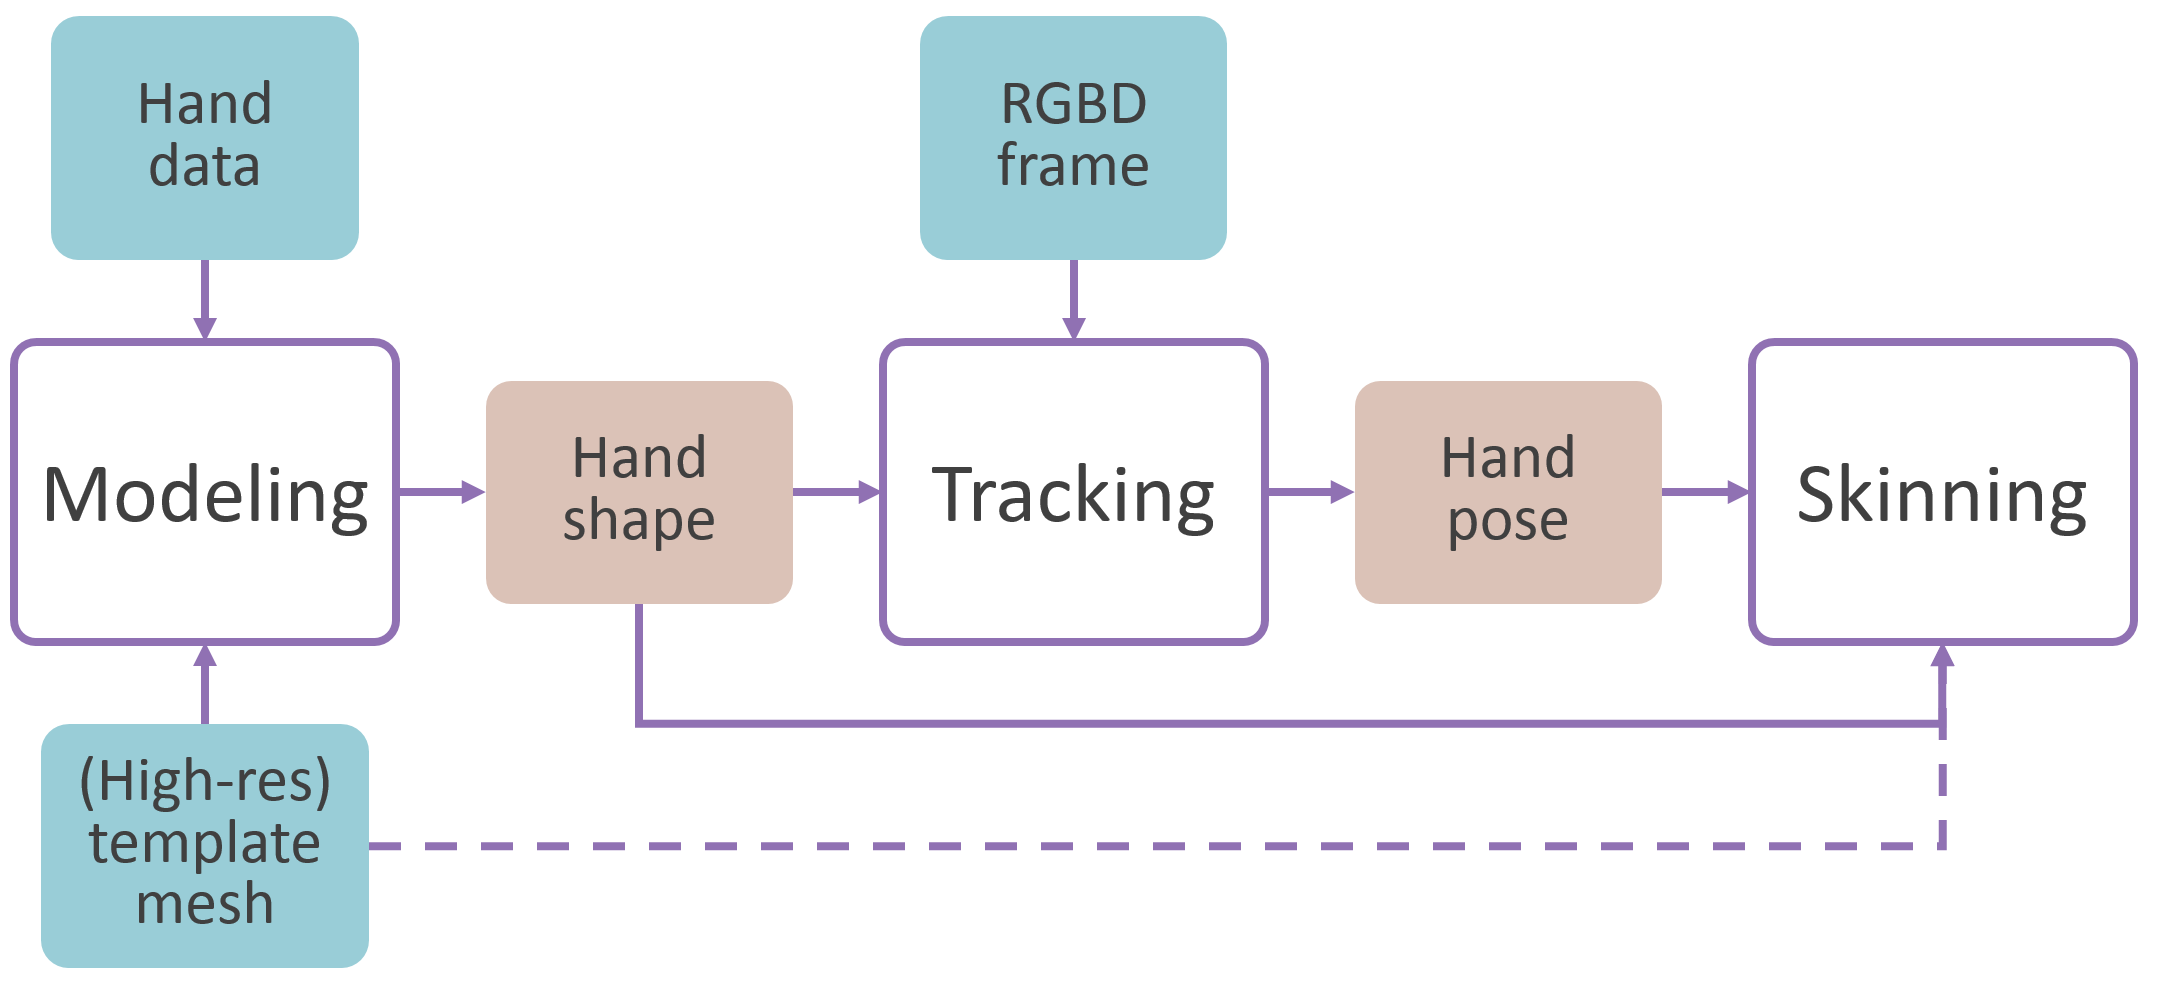
\includegraphics[width=0.5\textwidth]{fig/generic_pipeline}
	\caption{Generic pipeline for hand tracking. The input data that does not depend on the internal hand model representation is shown in blue, the representation-dependent components are shown in beige, and are listed in Table \ref{table:representation_dependent_components} for different representations.}
	\label{fig:generic_pipeline}
\end{figure}


\subsection{Why customizing the hand model?}

Hand model should be able to accurately represent the observed data.  The discrepancy between the optimal model pose given the data and the true hand pose can be significant, especially if the hand model does not reflect all the degrees of freedom of a hand (Figure \ref{fig:coarse_hand_model_and_lbs}, left).

\begin{figure}[h!] 
	\centering
	\hspace{-2em}
	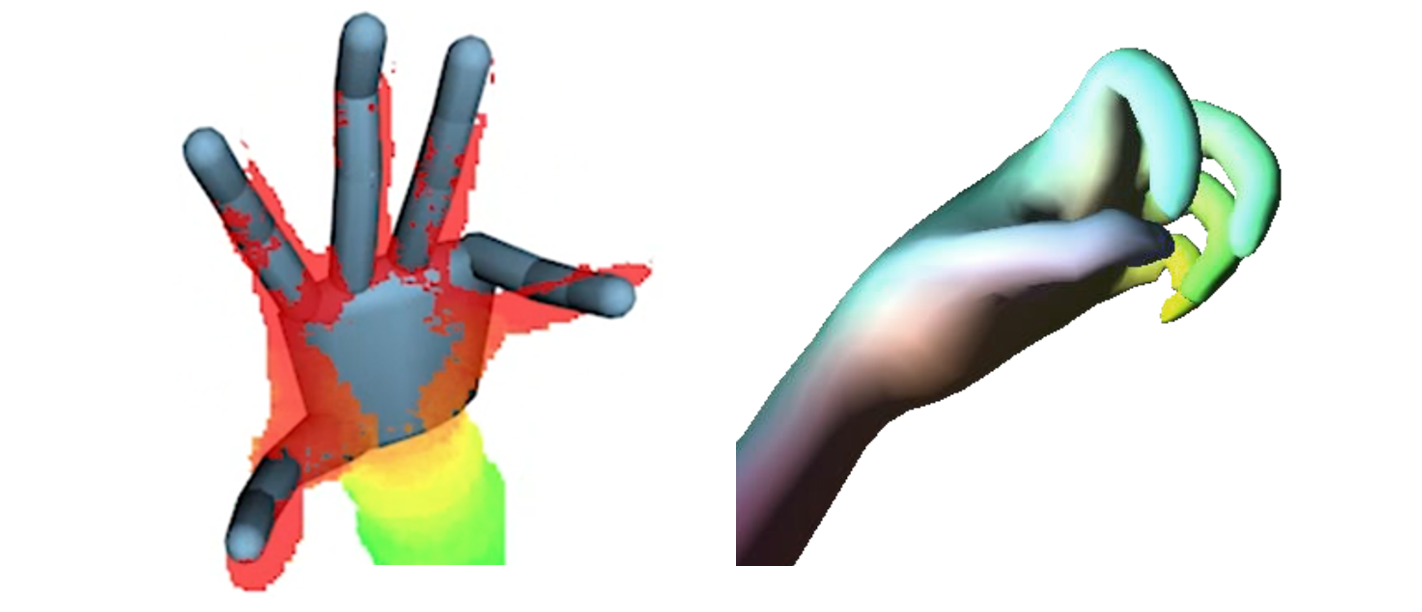
\includegraphics[width=0.5\textwidth]{fig/coarse_hand_model_and_lbs}
	\caption{Left - coarse hand model  from Tagliasacchi et. al.; right - hand model animated with linear blend skinning from Sharp e. al }.
	\label{fig:coarse_hand_model_and_lbs}
\end{figure}

\subsection{Why realistically animating the hand model?}

The hand skinning quality is obviously important for digital avatars applications. In AR and VR applications a 3D hand model can properly interact with 3D objects, establish a realistic contact and disappear behind them. Given that, the degree of immersion into virtual reality depends on whether a user sees own realistic hands \textcolor{mygray}{(find a study mentioned by Leap Motion).} The simple skinning approaches like linear blend skinning may generate implausible results  (Figure \ref{fig:coarse_hand_model_and_lbs}, right).

\subsection{Alternative hand model representations}
Each stage of the pipeline requires a hand model. There is several different hand model representations suggested by previous authors (see Figure \ref{fig:hand_model_representations}). Each representation is well suited for one of the stages, since it was used for the task on the first place. We argue that each representation also has weaknesses, which is why there exists a set of alternatives.

We suggest to use convolution surfaces representation of the hand model. 

Convolution surface is an implicit surface which is described by a control skeleton. The skeleton may consist of points, edges or polygons \cite{bloomenthal1991convolution}. In each vertex of the skeleton we define a radius. The radius in intermediate points is a linear combination of the radii at the neighboring vertices. Given the topology of the underlying skeleton, the model can be represented with convolution surface up to high precision \textcolor{mygray}{(find some theoretical estimates).} Next we present the arguments why convolution surfaces representation is suitable for all the stages of the pipeline.

\begin{table}[!ht] 
	\centering
	\begin{tabular}{|p{2.5cm}|p{2.5cm}|p{2.5cm}|}
	\hline
 	& Hand pose  & Hand shape  \\
	\hline
	Triangular mesh with embedded skeleton, \cite{taylor2014user} & Vertices and bones positions & Vertices and bones positions	 \\
	\hline
	Cylinder model, \cite{tagliasacchi2015robust} & Cylinders size and transformations & Cylinders transformations	 \\
	\hline
	Convolution surfaces model & Positions and radii of control points & Positions of control points \\
	\hline
	\end{tabular}
	\vspace{1em}
	\caption{Comparison of different hand model representations}
	\label{table:representation_dependent_components}
\end{table}

\subsection{Convolution surfaces for model fitting}
The spheres and mixed cylinders/spheres hand model representations (Figure \ref{fig:hand_model_representations} a, b) are ubiquitous in hand tracking, because they are well suited for tracking tack per se (see next) and can be quickly to created manually. If a small number of  building blocks is used, the precision of the model is low, especially in the palm region. A higher precision can be obtained by increasing the number of primitives, which defeats the purpose of model simplicity. Convolution surfaces representation gives higher precision for the same number of building blocks. \textcolor{mygray}{Add experimental or theoretical support for convolution surfaces.}
The triangles mesh representation can approximate the hand to a high precision. However, it is not trivial to specify the model parts that are rigid and should be kept the same shape between the poses. This results in overfitting to local skin deformations. 

\begin{figure}[h!] 
	\centering
	\hspace{-2em}
	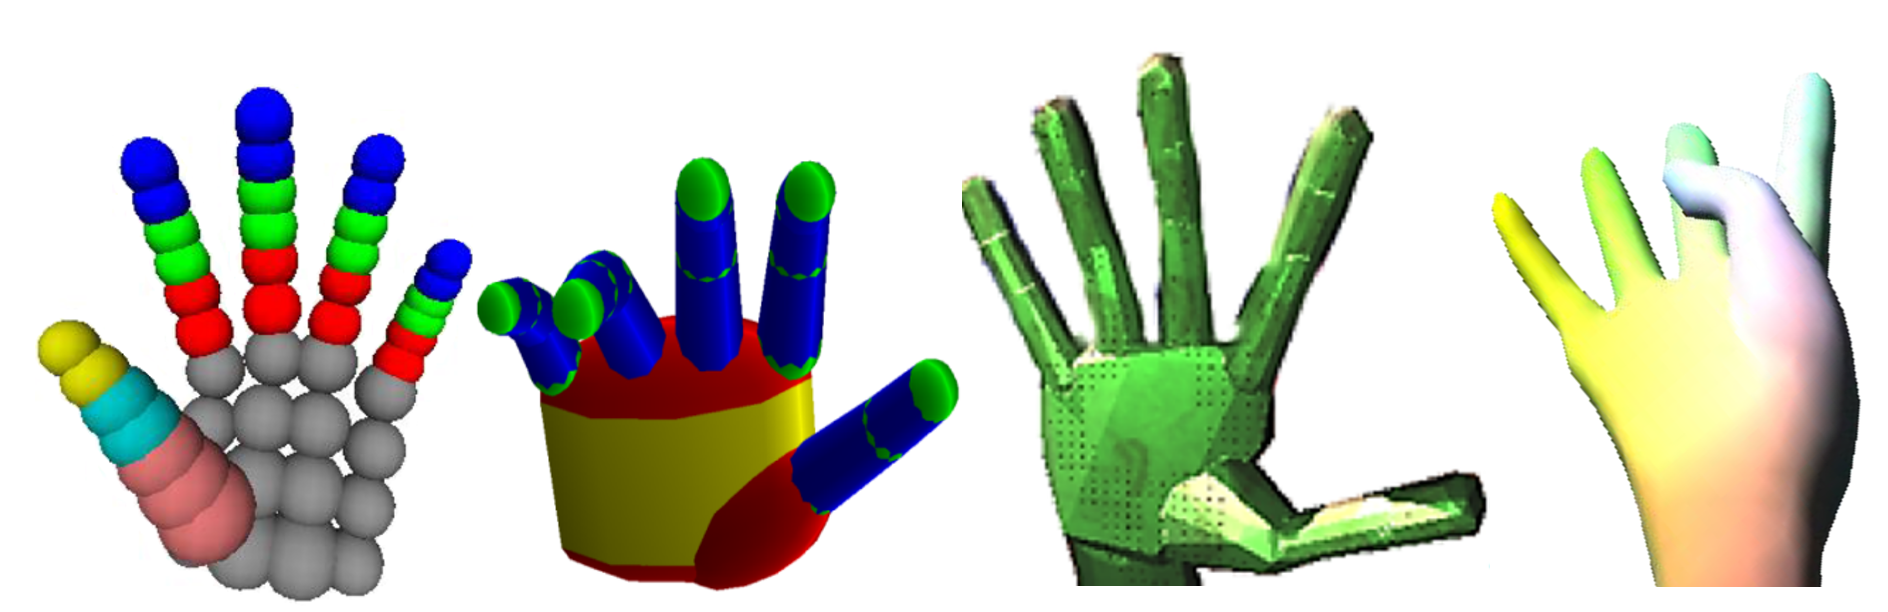
\includegraphics[width=0.5\textwidth]{fig/hand_model_representations}
	\caption {Hand model representations from works of (a) Qian et. al., (b)  Oikonomidis et. al., (c) Melax et. al.  and (d) Sharp et. al}
	\label{fig:hand_model_representations}
\end{figure}

\subsection{Convolution surfaces for hand tracking}
For model based tracking the main operation is to find the closest point on the model for a given data point. This operation is can be done in closed for each rigid segment with spheres/cylinder and convolution surfaces model representation. 
For a triangular mesh this operation has complexity linear in number of triangles. Thus, it is necessary to simplifying assumptions and/or more complex optimization to allow the hand tracking system to run in real time. (Look how different systems deal with this problem). Moreover, the triangular mesh has (much) more degrees of freedom than the underlying problem. Without additional regularization, rigid parts of the hand model can deform to fit the data and the individual vertices can shift to fit the sensor noise.

\subsection{Convolution surfaces for hand skinning}
The Linear Blend Skinning approach used to pose the triangular mesh model in previous works (\cite{sharp2015accurate}, \cite{schroder2013analysis} ) creates artifacts, the fingers looks like made from rubber. The spheres/cylinders model is not suitable for realistic animation, therefore a re-targeting step to a template mesh is required. Retargeting does not only demand additional effort, but also brings additional imprecision. The state of the art approaches in hand skinning are implicit surfaces-based (\cite{vaillant2013implicit},  \cite{vaillant2014robust} ).  A convolution surfaces model serves a ready to use input for such an approach.








